\section{PCB Editor} \label{sec:pcb_editor}



%%-------
\subsection{User Preferences} \label{ssec:user_preferences}

Опция параметра \textit{Effective} определяет точку применения: при активации, после рестарта, по~команде.

Опция параметра \textit{Favorite} позволяет добавить параметр на~вкладку избранное \textit{my\_favorites}.

\info{Приоритет поиска по~заданным в~параметрах путях "--- сверху вниз.}

\begin{tabularx}{\linewidth}{| m{6.5cm} | X |}
	\caption{Параметры \textit{User Preferences}} \label{tab:user_preferences} \\
	\hline	
	\calign{Название} 		& \calign{Описание} 					\\ \hline
	\endfirsthead
	
	\multicolumn{2}{r}{продолжение следует\ldots} 
	\endfoot
	\endlastfoot
	
	\multicolumn{2}{l}{Продолжение таблицы \ref{tab:user_preferences}} 					\\ \hline 
	\calign{Название} 		& \calign{Описание} 					\\ \hline
	\endhead
	
	\multicolumn{2}{|c|}{\textbf{Paths/Config}}						\\ \hline
	artpath					& Пути к~настройкам герберов.			\\ \hline
	viewpath				& Путь к~цветовым настройкам.			\\ \hline
	ncdpath					& Путь к~настройкам сверловки.			\\ \hline
	wizard\_template\_path	& Путь к~шаблонам ПП и символов (форм, механики, чертежей). \\ \hline
	
	\multicolumn{2}{|c|}{\textbf{Paths/Library}}					\\ \hline
	miscpath 				& Путь к~различным файлам, в~том~числе настройкам для экспорта в~*.dxf. \\ \hline
	modulepath 				& Путь к~смхемам повторного использования *.mdd. \\ \hline
	ncdpath 				& Путь к~настройкам сверловки.			\\ \hline
	padpath 				& Путь к~контактным площадкам.			\\ \hline
	parampath 				& Путь к~файлу настроек проекта (настройки цветов, сетки, трассировки). \\ \hline
	psmpath 				& Путь к~посадочным местам.				\\ \hline
	steppath 				& Путь к~3D~моделям.					\\ \hline
	techpath 				& Путь к~файлам технологических настроек (хранит также информацию о~слоях). \\ \hline
	topology\_template\_path& Путь к~файлам ограничений (материалы, проводимость). \\ \hline
	
	\multicolumn{2}{|c|}{Другие}									\\ \hline
	acon\_diag 				& Вне зависимости от~угла расположения элемента, трассировка начнется под~его углом. \\ \hline
	addline\_nomerge 		& Запрет связи двух линий при их соединении.	\\ \hline
	ads\_sdart 				& Путь для гербер файлов и файлов сверловки (по~умолчанию ложится в~проект). \\ \hline
	ads\_sdlog 				& Путь для log-файлов (по~умолчанию ложится в~проект). \\ \hline
	ads\_sdplot 			& Путь для plot файлов.					\\ \hline
	ads\_sdreport 			& Путь для отчетов.						\\ \hline
	allegro\_dynam\_timing	& \textcolor{red}{?!} 					\\ \hline
	allegro\_etch\_lenght\_on& Отображение текущей длинны проводника.\\ \hline
	autosave 				& Включение автосохранения.				\\ \hline
	autosave\_name			& Имя файла автосохранения.				\\ \hline
	autosave\_time			& Период автосохранения.				\\ \hline
	cancel\_key				& Клавиша полной отмены.				\\ \hline
	datatips\_delay 		& Задержка на~появление подсказки.		\\ \hline
	db\_tier\_nomsg 		& Сообщение об~ошибке версий БД.		\\ \hline
	dcnets\_delete\_norat	& Удаление свойства NO\_RAT для цепей питания.	\\ \hline
	disable\_opengl			& Отключение режима opengl.				\\ \hline
	display\_refdes\_rats	& Показывает привязку поз. обозначений.	\\ \hline
	draw\_etch\_outline		& Отображение границ линий.				\\ \hline
	dxf\_version			& Версия выходного *.dxf файла.			\\ \hline
	idf\_place\_bound\_bottom & \textcolor{red}{?!} 					\\ \hline
	idf\_place\_bound\_top	& \textcolor{red}{?!} 					\\ \hline
	idx\_place\_bound\_bottom & \textcolor{red}{?!} 				\\ \hline
	idx\_place\_bound\_top	& Слои для настройки высоты компонента.	\\ \hline
	logic\_edit\_enabled 	& Включение "Logic/Net logic" команд.	\\ \hline 
	max\_undo\_memory 		& Размер памяти отведенной под откаты.	\\ \hline
	modules\_no\_5x\_support& \textcolor{red}{?!}					\\ \hline
	nolast\_directory 		& \textcolor{red}{?!}					\\ \hline
	nolast\_file 			& \textcolor{red}{?!}					\\ \hline
	preserve\_symbol\_textblocks & \textcolor{red}{?!}				\\ \hline	
	step\_unsupported\_prototype & Включение опций поддержки 3D step-моделей. \\ \hline
%	symed\_pin\_names\_for\_voltage\_pins & \textcolor{red}{?!}		\\ \hline	
	undo\_depth 			& Количество откатов.					\\ \hline
	use\_accure\_delay\_calculation & Включение вычисления неравномерности экранирующего слоя. \\ \hline
\end{tabularx}



%%-------
\newpage
\subsection{3D модель} \label{ssec:3d_model}



%%%-------
\subsubsection{Привязка модели к посадочному месту} \label{sssec:step_package_mapping}

Подключить 3D модель, а~точнее STEP, к~посадочному месту можно выполнив следующие шаги:

\begin{enumerate}
	\item Скачать или создать STEP модель и~разместить ее по~доступному пути;
	\info{Доступный путь, это путь в~текущей папке символа или путь прописанный в~настройках \textit{<<User Preferences -> Paths -> Library -> steppath>>}.}
	
	\item Запустить \textbf{PCB Editor};
	
	\item Открыть файл посадочного места (*.dra) и~перейти в~окно \textit{<<Setup -> Step Package Mapping...>>};
	\info{Раньше этот пункт меню появлялся только после установки параметра \textit{<<step\_unsupported\_prototype>>} в~\textit{<<User Preferences>>}. В~версии \textbf{16.6 S032} такого параметра уже нет.}
	
	\item В~списке \textit{<<Available STEP Models>>} выбрать нужную модель элемента;
	
	\begin{figure}[H]
		\center{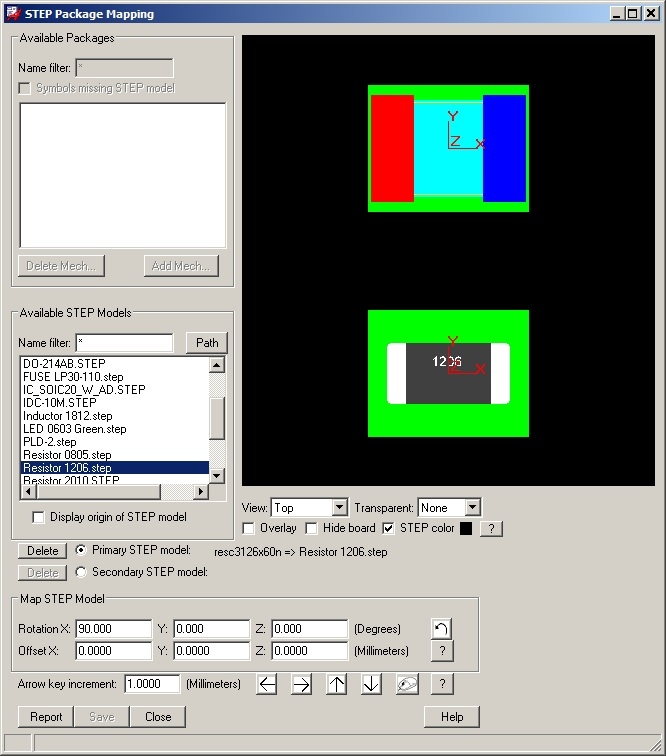
\includegraphics[width=0.5\linewidth]{step_model_mapping.jpg}}
%		\caption{Окно подключения \textbf{3D}~модели} 
%		\label{fig:step_model_mapping}
	\end{figure}
	
	\item При помощи поворотов и~сдвигов \textit{<<Map STEP Model>>} добиться нужного положения модели относительно контактных площадок. Правильность установки можно оценить переключая виды;
	\info{Посадочное место и~модель можно наложить друг на~друга, включив настройку \textit{<<Overlay>>}.}
	\info{Для удобства совмещения модели и~посадочного места, у~последнего точку привязки надо делать по~центру. По~крайней мере для многих моделей, что скачивал я, требовались лишь простейшие повороты, либо все сразу совпадало.} 
	\item Сохранить полученный результат. По~умолчанию это будет сделано в~\textit{<<./stepFaceFiles4Map/>>};
	
	\item В~дальнейшем при установке элемента на плату, он будет иметь 3D~изображение;
	
	\item В~итоге можно получить довольно приятную картинку платы, например как на~рисунке ниже.
	
	\begin{figure}[H]
		\center{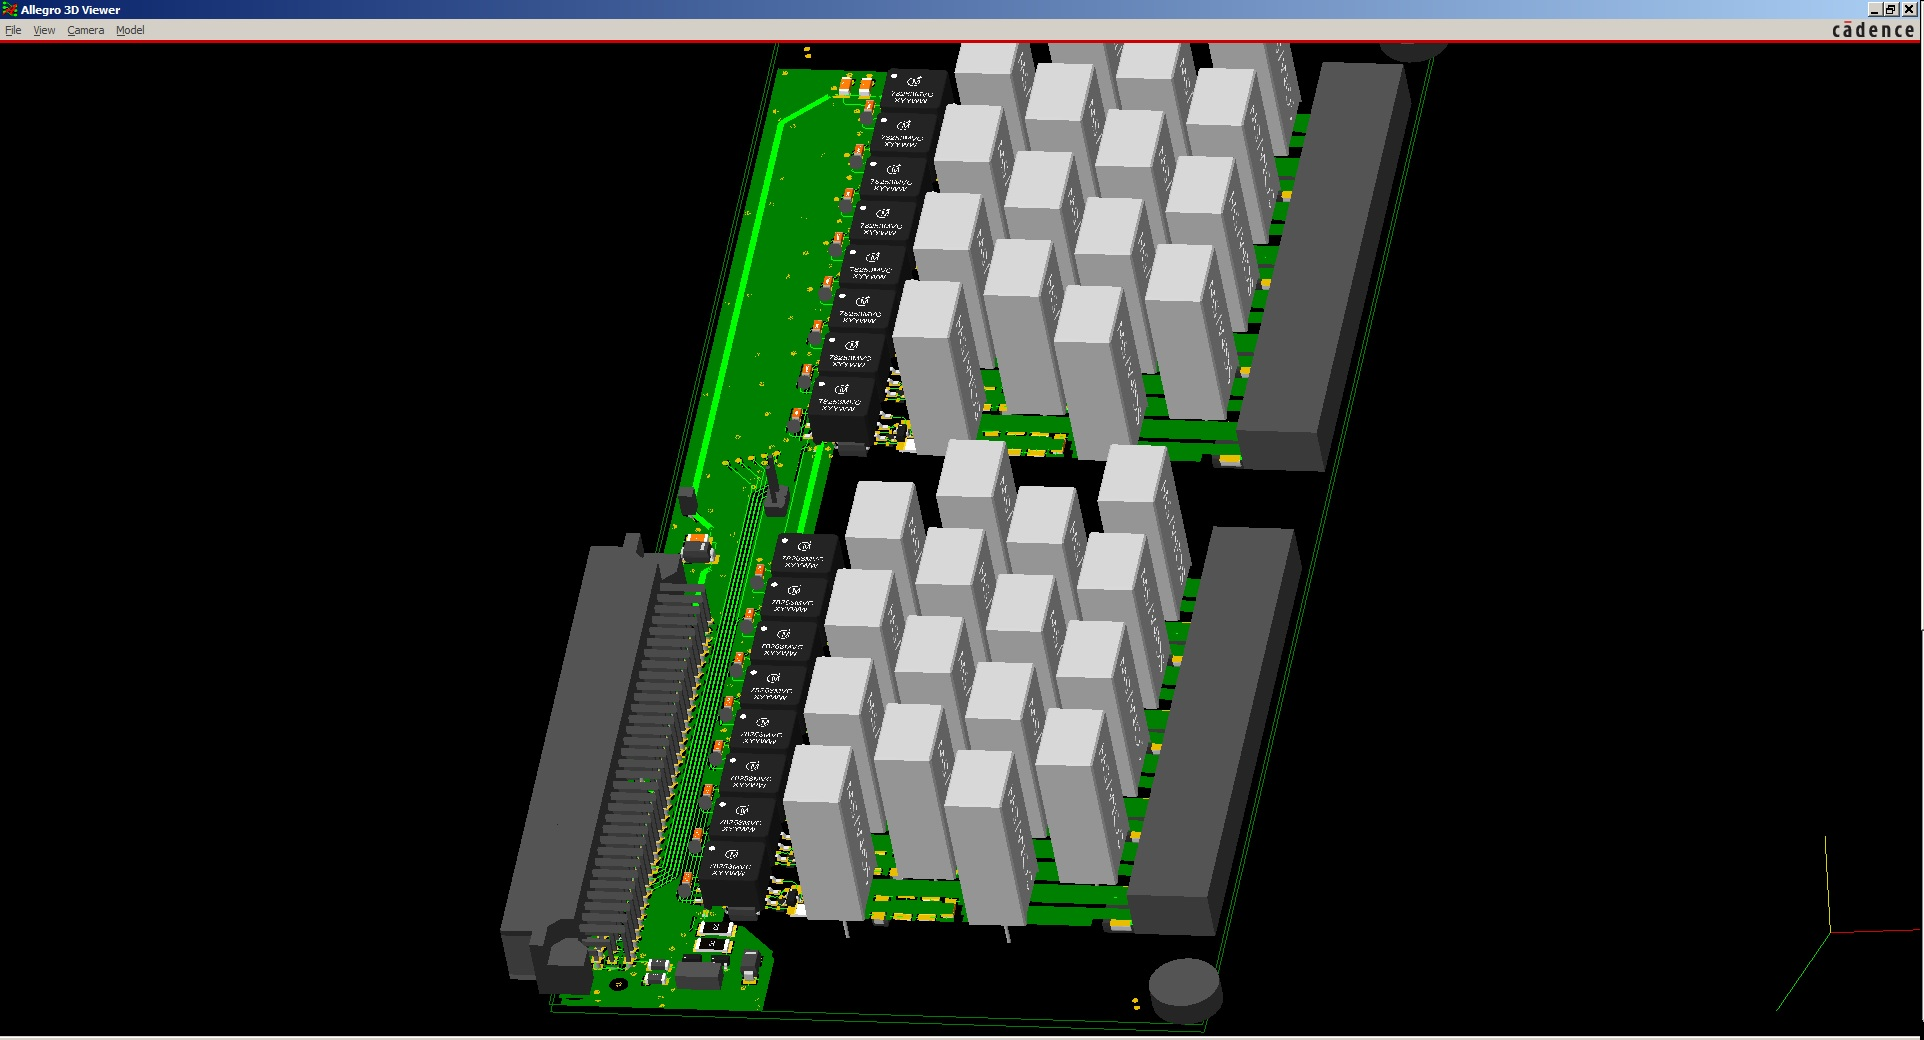
\includegraphics[width=0.8\linewidth]{example_3d_pcb.jpg}}
%		\caption{Пример платы с 3D моделями элементов} 
%		\label{fig:example_3d_pcb}
	\end{figure}
\end{enumerate}



%%-------
\newpage
\subsection{Надстройки} \label{ssec:pcb_plugin}



%%%-------
\subsubsection{Подключение} \label{sssec:pcb_plugin_setup}

Для подключения надстроек в~\textbf{PCB Editor} необходимо:
\begin{enumerate}
	\item Скопировать файлы в~папку \textit{<<\%CDS\_SITE\%/pcbenv/pcb/skil>>};
	\item Добавить загрузку надстроек в~файл \textit{allegro.init.txt} находящийся в той~же папке (либо создать его);
	\item В~зависимости от~надстройки, строка загрузки может принимать разный вид и необходимо ознакомиться с~приложенной к~ней документацией. Например, для \textbf{nsware} необходимо выполнить следующие действия:
	\begin{figure}[H]
		\center{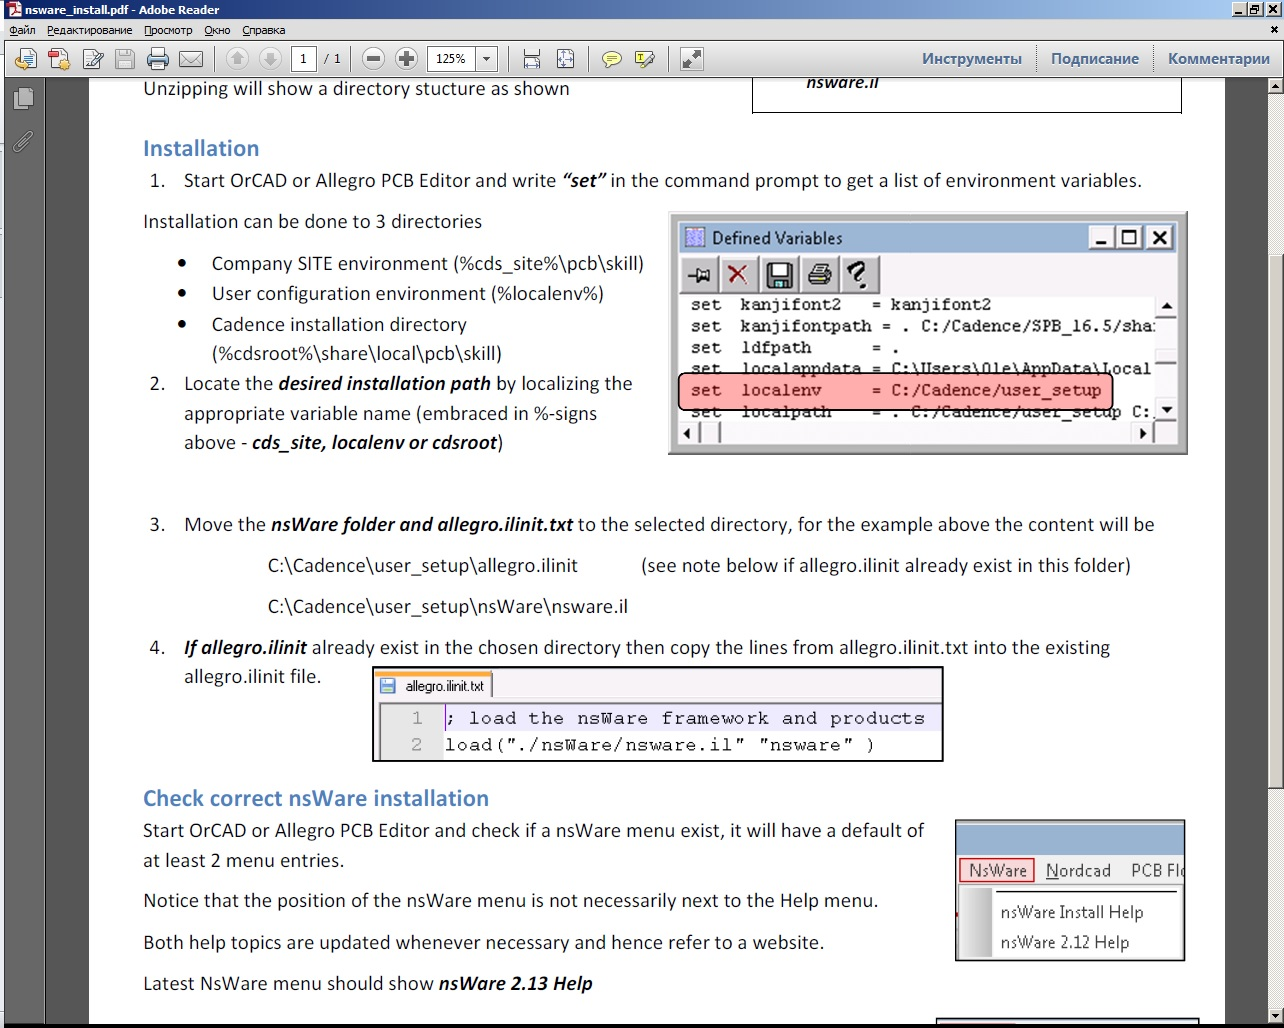
\includegraphics[width=0.8\linewidth]{nsware_plugin.jpg}}
%		\caption{Пример платы с 3D моделями элементов} 
%		\label{fig:example_3d_pcb}
	\end{figure}
	
	
	 
%%-------
\newpage
\subsection{Горячие кнопки} \label{ssec:hot_keys}
	 
	 Примеры горячих кнопок можно посмотреть в приложении \ref{app:hot_keys}.
	 
\end{enumerate}